% 2010 年陕西卷文科第 17 题：△ABC 中 D 在 BC 上，已知 ∠B=45°、AD=10、AC=14、DC=6。
% 来源 PDF：普通高考/2010/2010陕西文.pdf，SHA-256 428bcb4aee4c6a7a6a9c9d0dca1377b14112594015d1d50a931e725ae0c5c130。
% 原页：第 1 页（A3 三栏）第 3 栏下部，书页码 625。
% 重绘依据：照原页——B 在左下、C 在右下，BC 水平；A 在 BC 上方、位于 B 与 D 之间偏 D 一侧；
%   D 在 BC 上（介于 B、C 之间），连 AD、AC，只有 AB、AD、AC、BC 四条实线，无其他辅助线。
%   按题设取坐标（整体缩小 1/2.5）：B=(0,0)，A=(3.464,3.464)（∠B=45°），
%   D=(5.464,0)，C=(7.864,0)，此时 AD=4、DC=2.4、AC=5.6，与原图比例一致。
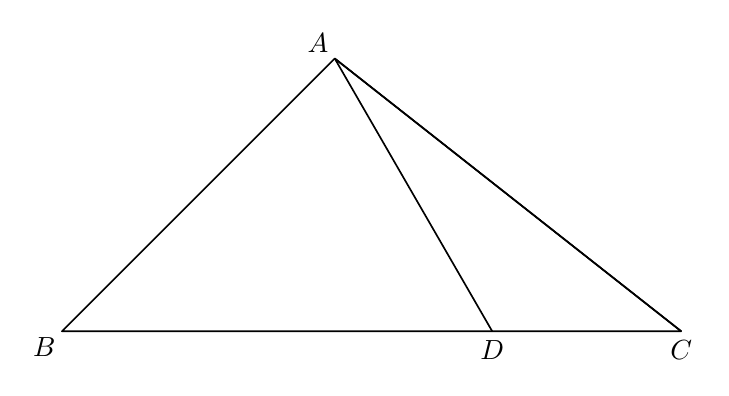
\begin{tikzpicture}[semithick, line join=round]
  \coordinate (B) at (0,0);
  \coordinate (C) at (7.864,0);
  \coordinate (D) at (5.464,0);
  \coordinate (A) at (3.464,3.464);

  \draw (A) -- (B) -- (C) -- cycle;
  \draw (A) -- (D);
  \draw (A) -- (C);

  \node[above left, inner sep=2pt] at (A) {$A$};
  \node[below left, inner sep=2pt] at (B) {$B$};
  \node[below, inner sep=3pt] at (C) {$C$};
  \node[below, inner sep=3pt] at (D) {$D$};
\end{tikzpicture}
